\usepackage[latin1]{inputenc}
\usepackage{array}
\usepackage{amsmath}
\usepackage{upgreek}
\usepackage{hyperref}

\usepackage{minted}
\usemintedstyle{perldoc}
\newmintedfile{c}{fontsize=\tiny, frame=lines, framesep=1mm}

\usepackage[absolute,overlay]{textpos}

\setbeamercolor{framesource}{fg=gray}
\setbeamerfont{framesource}{size=\tiny}

\newcommand{\source}[1]{\begin{textblock*}{4cm}(8.7cm,8.6cm)
    \begin{beamercolorbox}[ht=0.5cm,right]{framesource}
        \usebeamerfont{framesource}\usebeamercolor[fg]{framesource} Image Source: {#1}
    \end{beamercolorbox}
\end{textblock*}}

% \usepackage{minted}
% \usemintedstyle{perldoc}
% tiny, scriptsize, footnotesize, small, normalsize, large, Large, LARGE,
% huge Huge
% \newminted{d}    {fontsize=\tiny, frame=lines, framesep=1mm}
% \newminted{bash} {fontsize=\tiny, frame=lines, framesep=1mm}
% \newmintedfile{d}{fontsize=\tiny, frame=lines, framesep=1mm}

\usetheme[numbers, minimal]{NYU}
% Get rid of the navigation icons
\setbeamertemplate{navigation symbols}{}

\title{OpenCL/OpenGL Interoperation + MeshFree FEM}
\author{Julian Panetta}
\date{5 March 2013}
\begin{document}

\begin{frame}
\titlepage
\end{frame}

\section{OpenCL/OpenGL Interaction}
\begin{frame}{OpenGL}
    \begin{figure}
        
\includegraphics[width=.3 \textwidth]{images/ogl.jpg}
    \end{figure}
    \begin{itemize}
        \item Cross-platform API for visualization on the GPU
        \pause \item Includes shader languages (GLSL)
        \begin{itemize}
            \item Run code once per vertex, per rasterized pixel, etc.
            \pause \item Add great flexibliity on top of the traditional
                ``fixed function pipeline''
            \pause \item Can be tricked into doing some general purpose GPU
                  computing, but...
            \pause \item Computations like this tend to be hacks
        \end{itemize}
    \end{itemize}
\end{frame}

\begin{frame}{OpenCL}
    \begin{figure}
        
\includegraphics[width=.3 \textwidth]{images/opencl_logo.jpg}
    \end{figure}
    \begin{itemize}
        \item ``Open Computing Language:'' \\
              Simple C-like language for SIMD-type parallel programming
        \pause \item Generates vectorized code to run on:
            \begin{itemize}
                \item Multiple CPU cores
                \pause \item GPUs
                \pause \item Cell architectures, etc.
            \end{itemize}
        \pause \item Much better suited for computation than GLSL shaders
        \pause \item Often better-suited for vectorized CPU code (SSE, AVX) than C
              and/or intrinsics
    \end{itemize}
\end{frame}

\begin{frame}{OpenCL: Basic concept}
    \begin{figure}
        
\includegraphics[width=.3 \textwidth]{images/opencl_logo.jpg}
    \end{figure}
    \begin{itemize}
        \item Typical setting: you want to run a single operation on thousands
              of different inputs
        \pause \item Write a {\em kernel} program implementing the operation
        \pause \item Launch thousands of ``concurrent'' instances of the program, one
              per input
        \pause \item Examples
            \begin{itemize}
                \item 2D image convolution (OpenCL kernel implements convolution
                      kernel)
                \pause \item Eigenvalues of hundreds of 3x3 matrices
                \pause \item Many more: see your local HPC class
            \end{itemize}
    \end{itemize}
\end{frame}

\begin{frame}{Contexts}
    \begin{itemize}
        \item Both OpenGL and OpenCL have ``contexts''
        \pause \item OpenGL contexts manage:
            \begin{itemize}
                \item OpenGL state (transform matrices, rendering styles, etc.)
                \pause \item GLSL Programs
                \pause \item Memory buffers (vertex buffers, frame buffers, textures)
            \end{itemize}
        \pause \item OpenCL contexts manage:
            \begin{itemize}
                \item Kernels
                \pause \item Memory buffers
            \end{itemize}
    \end{itemize}
\end{frame}

\begin{frame}{Typical (GPU) OpenCL Program Flow}
    \begin{itemize}
        \item Create OpenCL context on a device (GPU)
        \pause \item Compile OpenCL Kernels
        \pause \item Allocate memory buffers on the GPU
        \pause \item Copy input data from CPU to GPU's input buffers
        \pause \item Run the kernel
        \pause \item {\color{red} Copy output data from the GPU's buffers back to the CPU}
        \pause \item {\color{red} Post-process (visualize?)}
    \end{itemize}
    \begin{itemize}
        \pause \item Transferring data to/from device adds significant overhead!
        \item Note: when the device is a CPU, all copies can be eliminated...
    \end{itemize}
\end{frame}

\begin{frame}[fragile]{OpenCL/OpenGL Context Interaction}
    \begin{figure}
        
\includegraphics[height=.2 \textwidth]{images/ogl.jpg}
        \raisebox{.1\textheight}{$\Longleftrightarrow$}
        
\includegraphics[height=.2 \textwidth]{images/opencl_logo.jpg}
    \end{figure}
    \begin{itemize}
        \item Ideally we'd leave the computation on the GPU for visualization.
        \pause \item We need OpenGL and OpenCL contexts to reference the same memory.
        \pause \item This memory could be VBOs (vertex buffers), textures on the OpenGL
              side.
        \pause \item We'll show how to have OpenCL write to a texture that OpenGL draws
              to the screen.
    \end{itemize}
\end{frame}

\begin{frame}{Sharing GPU Data: Overview}
    \begin{itemize}
        \item {\color{red} Create an OpenCL context on the same GPU, telling it to
            share with the active OpenGL context.}
        \pause \item {\color{blue} Allocate the texture with OpenGL calls (glGenTextures,
            etc.)}
        \pause \item {\color{blue} Create OpenCL ``buffers'' that just point to the
               OpenGL texture (clCreateFromGLTexture) }
        \pause \item {\color{green} Request OpenCL ownership of texture }
        \pause \item {\color{green} Run kernel, writing to the texture }
        \pause \item {\color{green} Release ownership of texture }
        \pause \item {\color{green} Render with OpenGL }
    \end{itemize}
\end{frame}

\begin{frame}{Sharing GPU Data: Context Creation}
    \begin{itemize}
        \item {\color{red} Create an OpenCL context on the same GPU, telling it to
            share with active OpenGL context.}
    \end{itemize}
    \pause This bit is platform dependent (Apple, WGL, GLX)
    \pause \cfile{snippets/context_apple.c}
\end{frame}

\begin{frame}{Sharing GPU Data: Buffer Allocation}
    \begin{itemize}
        \item {\color{blue} Allocate the texture with OpenGL calls (glGenTextures,
            etc.)}
        \item {\color{blue} Create OpenCL ``buffers'' that just point to the
               OpenGL texture (clCreateFromGLTexture) }
    \end{itemize}
    \pause \cfile{snippets/buffer_create.c}
\end{frame}

\begin{frame}{Sharing GPU Data: Visualization}
    \begin{itemize}
        \item {\color{green} Request OpenCL ownership of texture }
        \item {\color{green} Run kernel, writing to the texture }
        \item {\color{green} Release ownership of texture }
        \item {\color{green} Render with OpenGL }
    \end{itemize}
    \pause \cfile{snippets/run_vis.c}
    \begin{itemize}
        \pause \item glFinish/clFinish ensure GL/CL commands each finish before the
              other is run
        \pause \item Benchmark warning: without glFinish, clEnqueueAcquireGLObjects takes non-negligible
            time
    \end{itemize}
\end{frame}

\begin{frame}{Sharing GPU Data: The Kernel}
    \begin{itemize}
        \item The OpenCL buffer bound to the texture is of type
            \texttt{image2d\_t}
        \pause \item must use \texttt{write\_imagef} to write to the texture.
    \end{itemize}
    \cfile{snippets/kernel.cl}
\end{frame}

\begin{frame}{Demo: OpenCL Mandelbrot Viewer}
    \begin{figure}
        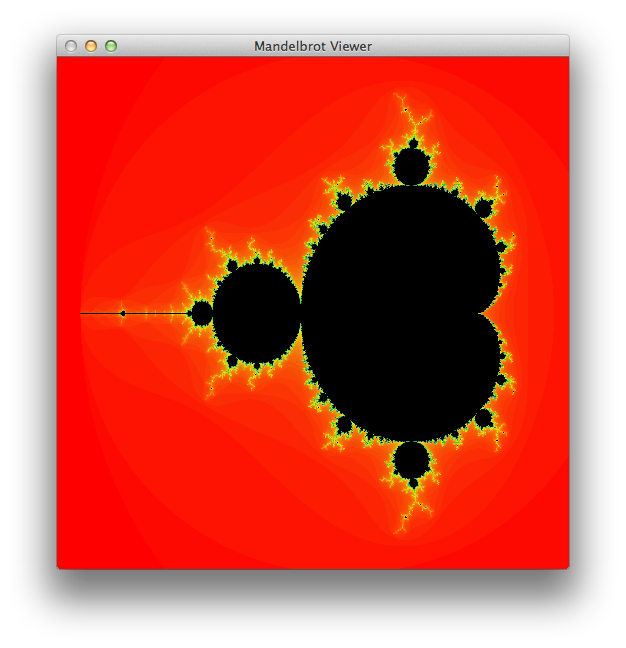
\includegraphics[width=.6 \textwidth]{images/mandelbrot_demo.png}
    \end{figure}
    \begin{center}
    Demo
    \end{center}
\end{frame}

\begin{frame}{Mesh-free FEM}
    \begin{itemize}
        \item James recently described our work on structural analysis.
        \item Pipeline:
            \begin{figure}
                
\includegraphics[width=.9\textwidth]{images/algorithm_overview.pdf}
            \end{figure}
        \pause \item Missing initial stage: volume meshing!
        \pause \item There are several reasons to want to avoid meshing.
    \end{itemize}
\end{frame}

\begin{frame}{Mesh-free FEM: Why?}
    \begin{itemize}
        \item Complicated geometry can be hard to mesh robustly.
            \begin{figure}
                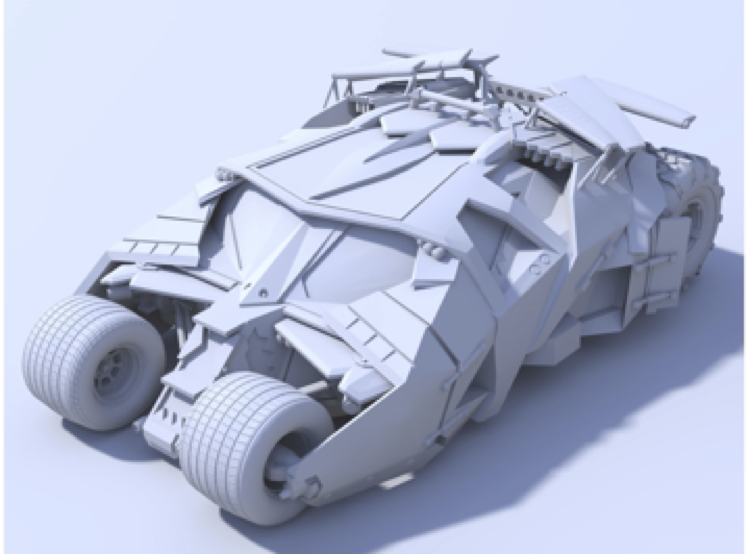
\includegraphics[width=.3\textwidth]{images/batmobile.png}
            \end{figure}
        \pause \item Free ourselves from the surface resolution (we might want
                     to coarsen some areas).
        \pause \item Sometimes you don't even have a mesh (CSG)
            \begin{figure}
                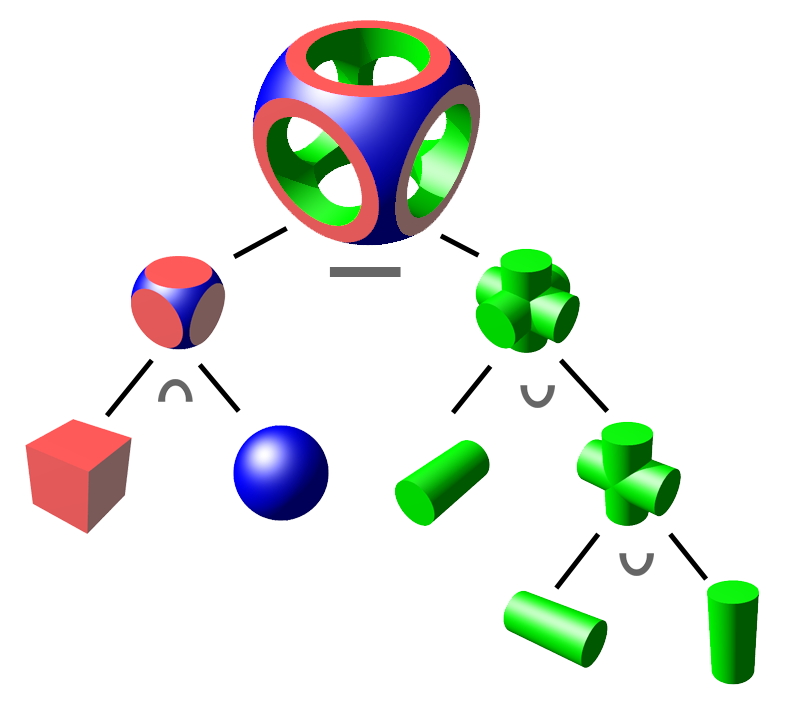
\includegraphics[width=.3\textwidth]{images/csg_tree.png}
                \source{Wikipedia}
            \end{figure}
    \end{itemize}
\end{frame}

\begin{frame}{Mesh-free FEM: What?}
    \begin{itemize}
        \item Use FEM discretization, but only require inside/outside geometry
              point queries
        \pause \item There *is* still a mesh: a regular grid.
            \begin{figure}
                
\includegraphics[width=.4\textwidth]{images/meshfree.png}
            \end{figure}
        \pause \item Note: doesn't conform to the object's boundary.
    \end{itemize}
\end{frame}

\begin{frame}{Mesh-free FEM: Details}
    \begin{figure}
        
\includegraphics[width=.2\textwidth]{images/meshfree.png}
    \end{figure}
    \begin{itemize}
        \item Elements are grid cells overlapping the object.
        \pause \item Bilinear basis functions interpolate DoFs on the element corners.
        \pause \item Strain is no longer piecewise constant! Integrals get trickier.
        \pause \item Integrands are not continuous on boundary cells (defined to be
            zero outside object) $\Longrightarrow$ many quadrature points needed
    \end{itemize}
\end{frame}

\begin{frame}{Mesh-free FEM: Challenges}
    \begin{itemize}
        \item Visualization
            \begin{itemize}
                \pause \item FEM equations yield values on grid, not geometry vertices
                \pause \item Displacement fields must be used to deform the geometry
                      somehow...
                \pause \item Solution: Fancy GLSL shader warping texture coordinates
            \end{itemize}
        \pause \item Boundary cells without enough quadrature points... (see Demo)
        \pause \item Boundary conditions!
            \begin{itemize}
                \item Boundaries don't have explicit representation, so
                    applying Dirichlet/Neumann boundary conditions is tricky
                \pause \item We have only Neumann conditions: traction applied to the
                      surface
                \pause \item We plan to blur the surface forces to convert them into
                      volume forces that can be integrated over the cells
            \end{itemize}
    \end{itemize}
\end{frame}

\begin{frame}{Implementation: CSGFEM}
    \begin{itemize}
    \item Apply structural analysis to CSG trees:
    \begin{figure}
        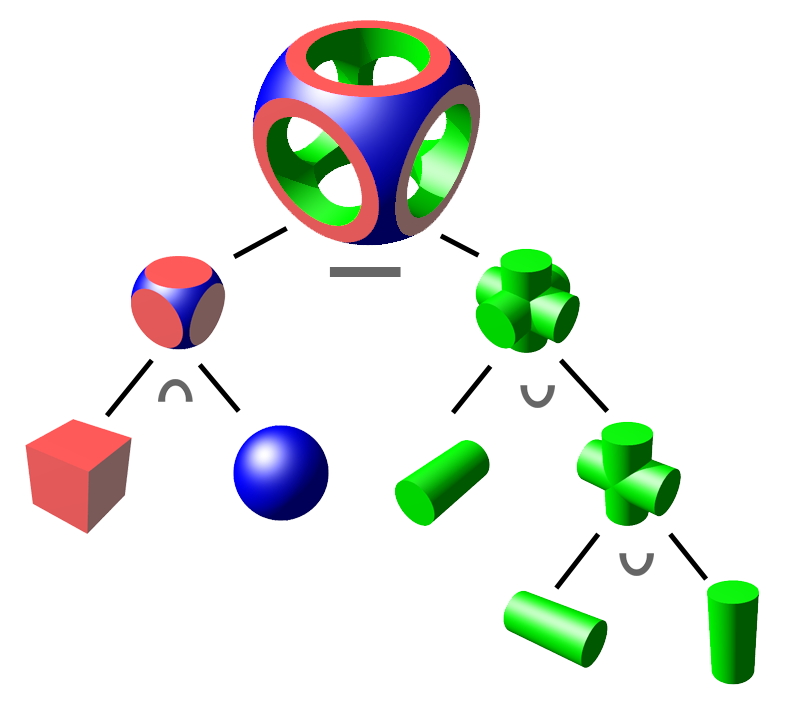
\includegraphics[width=.3\textwidth]{images/csg_tree.png}
        \source{Wikipedia}
    \end{figure}
    \pause \item Render geometry to texture using OpenCL
        \begin{itemize}
        \item Note: can't use recursion!
        \end{itemize}
    \pause \item Visualize deformations using GLSL/OpenGL
    \pause \item Currently have modal analysis working...
    \end{itemize}
\end{frame}

\begin{frame}{Demo: Mesh-free FEM}
    \begin{figure}
        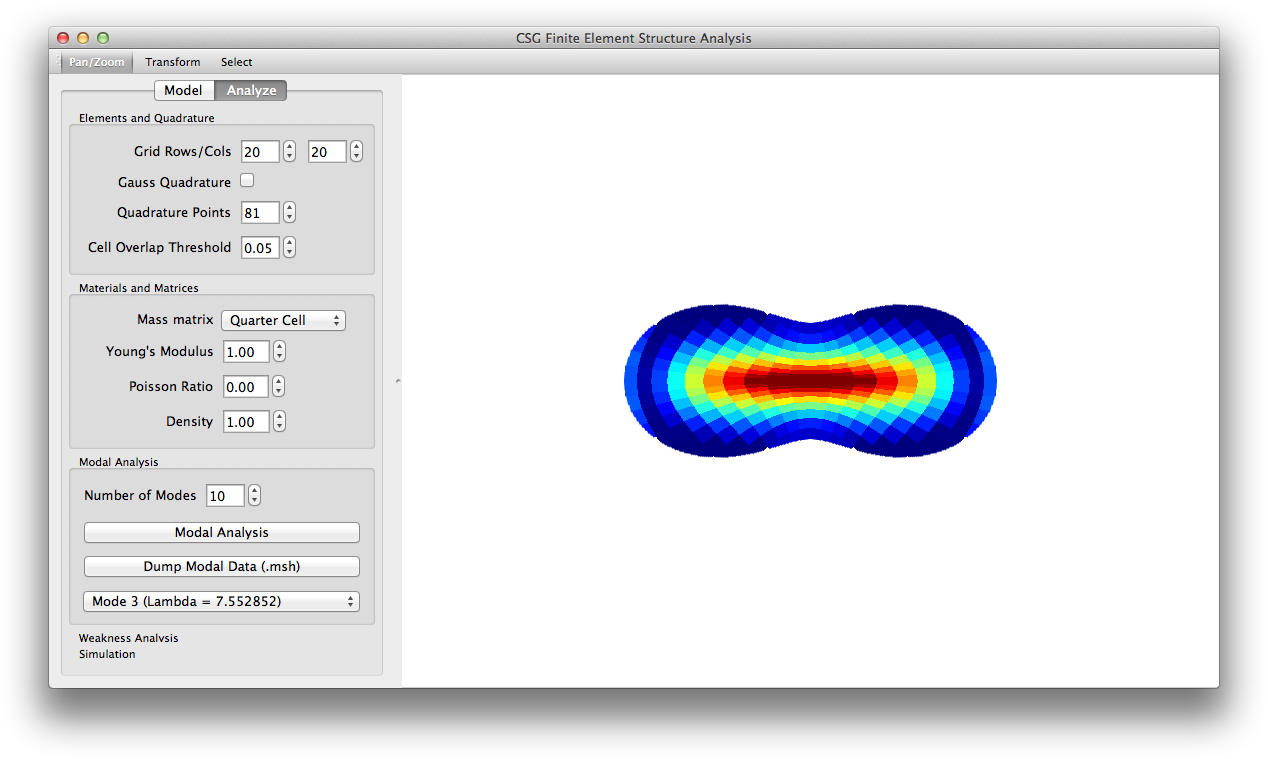
\includegraphics[width=.9 \textwidth]{images/csgfem_demo.png}
    \end{figure}
    \begin{center}
    Demo
    \end{center}
\end{frame}

\end{document}
